\documentclass{article}
%% \usepackage[T1]{fontenc} 
\usepackage[utf8]{inputenc}
\usepackage{Sweave}
\usepackage{thumbpdf}
\usepackage{url}
\usepackage{hyperref}
\usepackage{mathrsfs, amsmath, amsfonts, amssymb, amsthm}
%\usepackage[left=2.5cm,right=2.5cm]{geometry}
\usepackage{graphicx}
%\usepackage{draftwatermark}
\hypersetup{
  colorlinks=true,
  pdftitle={Reserving based on log-incremental payments in R},%
  pdfauthor={Markus Gesmann}%
}


%\VignetteIndexEntry{Reserving based on log-incremental payments in R}
%\VignetteDepends{ChainLadder}
%\VignetteKeywords{Claims, reserving, IBNR, chain ladder, stochastic reserving, statistical software}
%\VignettePackage{ChainLadder}



\setlength{\parindent}{0.0in}
\setlength{\parskip}{2mm}
\setlength{\headsep}{0.05in}
\setlength{\tabcolsep}{1.5pt}

\newcommand{\chainladder}{\textbf{\texttt{ChainLadder}} }
% Change default font to a sans serifs
\renewcommand{\familydefault}{\sfdefault}

\begin{document}
\Sconcordance{concordance:Log-incremental.tex:Log-incremental.Rnw:%
1 23 1 1 7 29 1 1 4 22 1 1 2 1 0 1 9 11 0 1 2 3 1 1 7 20 0 1 2 9 1 1 2 %
15 0 1 2 1 1 1 2 7 0 2 2 4 0 2 2 1 0 1 7 6 0 1 2 1 0 1 1 3 0 1 2 2 1 1 %
-4 1 8 7 1 1 2 1 0 1 2 4 0 1 2 2 1 1 -4 1 8 53 1 1 2 1 0 1 1 1 6 8 0 1 %
2 2 1 1 2 1 0 1 4 3 0 2 1 12 0 1 2 3 1 1 20 22 0 1 2 6 1 1 -8 1 12 44 1 %
1 11 1 2 28 1 1 5 7 0 1 9 7 1 1 -9 1 13 9 1 1 5 7 0 1 2 5 1 1 2 30 0 1 %
2 8 1 1 5 4 0 1 1 25 0 1 2 6 1 1 2 1 0 2 1 3 0 1 2 5 1 1 2 10 0 1 2 3 1 %
1 -14 1 18 14 1 1 18 20 0 1 3 4 0 1 2 2 1 1 -4 1 8 8 1 1 4 3 0 1 1 26 0 %
1 3 4 0 1 2 10 1 1 -12 1 16 17 1 1 23 25 0 1 2 7 1 1 2 1 0 1 4 3 0 1 9 %
11 0 2 2 1 0 1 1 6 0 2 1 7 0 1 2 5 1 1 2 15 0 1 2 5 1 1 3 14 0 1 2 23 1}


\author{Markus Gesmann}

\title{Reserving based on log-incremental payments in R}
\maketitle
\begin{abstract}

 paper Regression models based on log-incremental payments by Stavros Christofides [1], published as part of the Claims Reserving Manual (Version 2) of the Institute of Actuaries.

The paper is available together with a spread sheet model, illustrating the calculations. It is very much based on ideas by Barnett and Zehnwirth, see [2] for a reference. However, doing statistical analysis in a spread sheet programme is often cumbersome. I will go through the first 15 pages of Christofides' paper today and illustrate how the model can be implemented in R. 
  
\end{abstract}

\clearpage
\tableofcontents
\clearpage



\section{Development triangles}\label{sec:triangles}

Historical insurance data is often presented in form of a triangle
structure, showing the development of claims over time for each
exposure (origin) period. An origin period could be the year the
policy was written or earned, or the loss occurrence period. Of course the
origin period doesn't have to be yearly, e.g. 
quarterly or monthly origin periods are also often used. 
The development period of an origin period is also called age or lag.
Data on the diagonals present payments in the same calendar period.
Note, data of individual policies is usually aggregated to homogeneous 
lines of business, division levels or perils.

As an example we present a claims payment triangle from a UK Motor
Non-Comprehensive account as published by~\cite{Christofides1997}. For
convenience we set the origin period from 2007 to 2013.

The following data frame presents the claims data in a typical form as
it would be stored in a data base. The first column holds the origin
year, the second column the development year and the third
column has the incremental payments / transactions.

\begin{Schunk}
\begin{Sinput}
R> n <- 7
R> Claims <- 
     data.frame(originf = factor(rep(2007:2013, n:1)),
                dev=sequence(n:1),
                inc.paid= 
                c(3511, 3215, 2266, 1712, 1059, 587, 
                  340, 4001, 3702, 2278, 1180,  956,
                  629, 4355, 3932, 1946, 1522, 1238, 
                  4295, 3455, 2023, 1320, 4150, 3747, 
                  2320, 5102, 4548, 6283))
\end{Sinput}
\end{Schunk}
To present the data in a triangle format we can use the \texttt{matrix}
function: % of the \texttt{reshape2} package:
%% library(reshape2)
%% (inc.triangle  <- acast(Claims, origin ~ dev , value.var='inc.paid'))
\begin{Schunk}
\begin{Sinput}
R> (inc.triangle  <- with(Claims, {
     M <- matrix(nrow=n, ncol=n, 
                 dimnames=list(origin=levels(originf), dev=1:n))
     M[cbind(originf, dev)] <- inc.paid
     M
   }))
\end{Sinput}
\begin{Soutput}
      dev
origin    1    2    3    4    5   6   7
  2007 3511 3215 2266 1712 1059 587 340
  2008 4001 3702 2278 1180  956 629  NA
  2009 4355 3932 1946 1522 1238  NA  NA
  2010 4295 3455 2023 1320   NA  NA  NA
  2011 4150 3747 2320   NA   NA  NA  NA
  2012 5102 4548   NA   NA   NA  NA  NA
  2013 6283   NA   NA   NA   NA  NA  NA
\end{Soutput}
\end{Schunk}
It is the objective of a reserving exercise to forecast the future claims
development in the bottom right corner of the triangle and potential
further developments beyond development age 7. Eventually all claims
for a given origin period will be settled, but it is not always
obvious to judge how many years or even decades it will take. We speak
of long and short tail business depending on the time it takes to pay
all claims. 

Often it is helpful to consider the cumulative development of claims
as well, which is presented below.  
\begin{Schunk}
\begin{Sinput}
R> (cum.triangle <- t(apply(inc.triangle, 1, cumsum)))
\end{Sinput}
\begin{Soutput}
      dev
origin    1    2     3     4     5     6     7
  2007 3511 6726  8992 10704 11763 12350 12690
  2008 4001 7703  9981 11161 12117 12746    NA
  2009 4355 8287 10233 11755 12993    NA    NA
  2010 4295 7750  9773 11093    NA    NA    NA
  2011 4150 7897 10217    NA    NA    NA    NA
  2012 5102 9650    NA    NA    NA    NA    NA
  2013 6283   NA    NA    NA    NA    NA    NA
\end{Soutput}
\end{Schunk}
The latest diagonal of the triangle presents the latest cumulative paid 
position of all origin years:
\begin{Schunk}
\begin{Sinput}
R> (latest.paid <- cum.triangle[row(cum.triangle) == n - col(cum.triangle) + 1])
\end{Sinput}
\begin{Soutput}
[1]  6283  9650 10217 11093 12993 12746 12690
\end{Soutput}
\end{Schunk}
We add the cumulative paid data as column to the data frame as well.
\begin{Schunk}
\begin{Sinput}
R> Claims$cum.paid <- cum.triangle[with(Claims, cbind(originf, dev))]
\end{Sinput}
\end{Schunk}
To start the reserving analysis we plot the data.
\begin{Schunk}
\begin{Sinput}
R> op <- par(fig=c(0,0.5,0,1), cex=0.8, oma=c(0,0,0,0))
R> with(Claims, {
     interaction.plot(x.factor=dev, trace.factor=originf, response=inc.paid, 
                      fun=sum, type="b", bty='n', legend=FALSE); axis(1, at=1:n)
     par(fig=c(0.45,1,0,1), new=TRUE, cex=0.8, oma=c(0,0,0,0))
     interaction.plot(x.factor=dev, trace.factor=originf, response=cum.paid, 
                      fun=sum, type="b", bty='n'); axis(1,at=1:n)
   })
R> mtext("Incremental and cumulative claims development", 
         side=3, outer=TRUE, line=-3, cex = 1.1, font=2)
R> par(op)
\end{Sinput}
\end{Schunk}
\begin{figure}[thb]
  \begin{center}
  \setkeys{Gin}{width=0.75\textwidth}
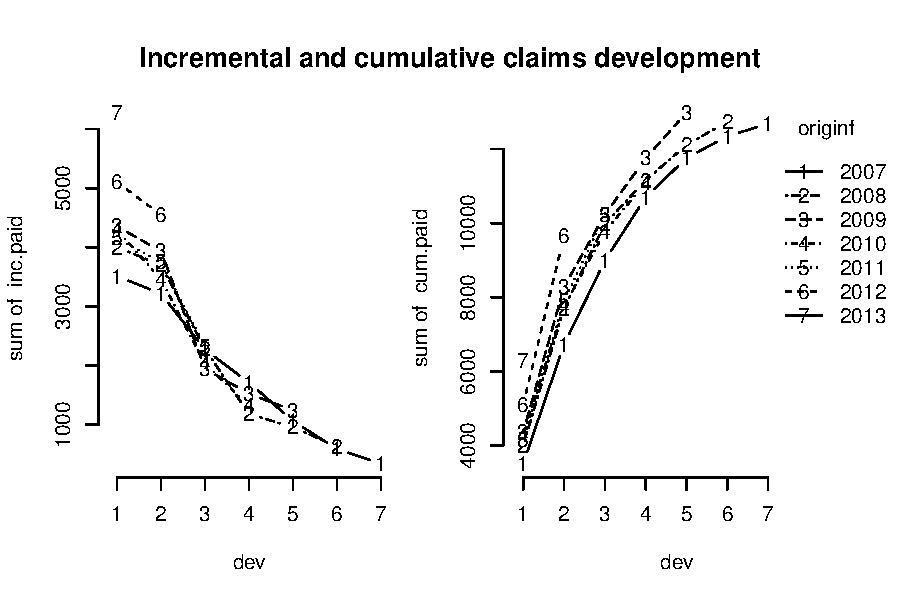
\includegraphics{Log-incremental-triangleplotinteractionplot}
\caption{Plot of incremental and cumulative claims payments by origin
  year using base graphics, using \texttt{interaction.plot} of the 
  \texttt{stats} package in \textsf{R}.}
\label{fig:triangleinteraction}
\end{center}
\end{figure}


\begin{Schunk}
\begin{Sinput}
R> library(lattice)
R> xyplot(cum.paid ~ dev | originf, data=Claims, t="b", layout=c(4,2),
          as.table=TRUE, main="Cumulative claims development")
\end{Sinput}
\end{Schunk}
\begin{figure}[thb]
  \begin{center}
  \setkeys{Gin}{width=0.75\textwidth}
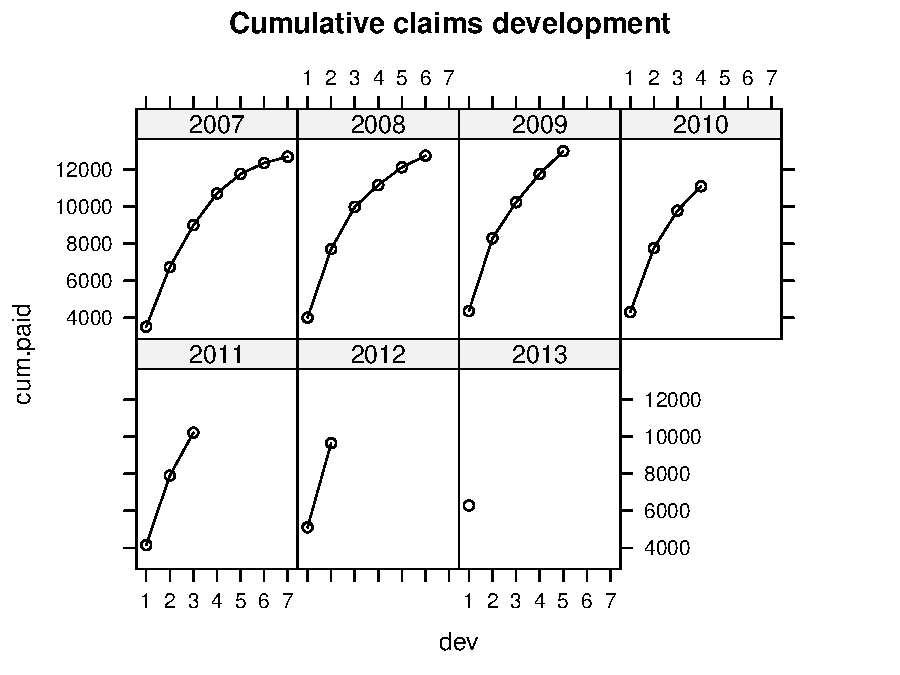
\includegraphics{Log-incremental-triangleplotlattice}
\caption{Claims developments by origin year using the
  \texttt{lattice} package, with one panel per origin year.}
\label{fig:trianglelattice}
\end{center}
\end{figure}
Figures~\ref{fig:triangleinteraction} and~\ref{fig:trianglelattice}
present the incremental and cumulative claims development by origin
year. The triangle appears to be fairly well behaved. The last two years, 
2012 and 2013 appear to be slightly higher than years 2008 to 2011  and the
values in 2007 are lower in comparison to the later years, e.g. 
the book changed over the years. The last
payment of 1,238 for the 2009 origin year stands out a bit as well. 

Other claims information can provide valuable insight into the
reserving process too, such as claims numbers, transition timings between 
different claims settlement stages and earning patterns. See for
example~\cite{MariaDoloresMartinezMiranda2011, Orr2007, Murray2011} 
respectively. A deep understanding of the whole business process from pricing,
underwriting, claims handling and data management will guide the
actuary to interpret the claims data at hand. 
The Claims Reserving Working Party Paper, \cite{ClaimsReservingWorkingParty:2002},
outlines the different aspects in more detail.



\subsection{Chain-ladder in the context of linear regression}

Since the early 1990s several papers have been published to embed the
deterministic chain-ladder method into a statistical framework. 
\cite{ZehnwirthBarnettProceedings, DanielMurphy1994} were not the only ones to 
point out that the chain-ladder age-to-age link ratios could be regarded as 
coefficients of a linear regression through the origin. To illustrate this 
concept we follow~\cite{ZehnwirthBarnettProceedings}. 

Let $C_{\cdot,k}$ denote the $k$-th column in the cumulative claims triangle. 
The chain-ladder algorithm can be seen as: 
\begin{align}
 C_{\cdot,k + 1} &  = f_k\, C_{\cdot, k} + \varepsilon(k) \mbox{ with }
 \varepsilon_{k} \sim N(0, \sigma_k^2 C_{\cdot, k}^\delta)
\end{align}
The parameter $f_k$ describes the slope or the 'best' line through
the origin and data points $[C_{\cdot,k}, C_{\cdot, k+1}]$, with
$\delta$ as a 'weighting' parameter.  \cite{ZehnwirthBarnettProceedings}
distinguish the cases: 
\begin{itemize}
\item $\delta = 0$ ordinary regression with intercept $0$
\item $\delta = 1$ historical chain ladder age-to-age link ratios
\item $\delta = 2$ straight averages of the individual link ratios
\end{itemize}
Indeed, we can demonstrate the different cases by applying different
linear models to our data. First, we add columns to the original data
frame \texttt{Claims}, to have payments of the current and previous
development period next to each other, additionally we add a column with 
the development period as a factor.
\begin{Schunk}
\begin{Sinput}
R> names(Claims)[3:4] <- c("inc.paid.k", "cum.paid.k")
R> ids <- with(Claims, cbind(originf, dev))
R> Claims <- within(Claims,{
     cum.paid.kp1 <- cbind(cum.triangle[,-1], NA)[ids]
     inc.paid.kp1 <- cbind(inc.triangle[,-1], NA)[ids]
     devf <- factor(dev)
     }
   )
\end{Sinput}
\end{Schunk}
In the next step we apply the linear regression function \texttt{lm} to each 
development period, vary the weighting parameter $\delta$ from 0 to 2 and 
extract the slope coefficients.
\begin{Schunk}
\begin{Sinput}
R> delta <- 0:2
R> ATA <- sapply(delta, function(d)
     coef(lm(cum.paid.kp1 ~ 0 + cum.paid.k : devf, 
        weights=1/cum.paid.k^d, data=Claims))
   )
R> dimnames(ATA)[[2]] <- paste("Delta = ", delta)
R> ATA
\end{Sinput}
\begin{Soutput}
                 Delta =  0 Delta =  1 Delta =  2
cum.paid.k:devf1      1.888      1.889      1.890
cum.paid.k:devf2      1.280      1.282      1.284
cum.paid.k:devf3      1.146      1.147      1.148
cum.paid.k:devf4      1.097      1.097      1.097
cum.paid.k:devf5      1.051      1.051      1.051
cum.paid.k:devf6      1.028      1.028      1.028
\end{Soutput}
\end{Schunk}
Indeed, the development ratios for $\delta=1$ and $\delta=2$ tally with those 
of the previous section. Let's plot the data again, with the cumulative paid
claims of one period against the previous one, including the regression output
for each development period, see Figure~\ref{fig:linearregression}. 
\begin{Schunk}
\begin{Sinput}
R> xyplot(cum.paid.kp1 ~ cum.paid.k | devf, 
          data=subset(Claims, dev < (n-1)), 
          main="Age-to-age developments", as.table=TRUE, 
          scales=list(relation="free"), 
          key=list(columns=2, lines=list(lty=1:4, type="l"), 
                   text=list(lab=c("lm(y ~ x)",
                                   "lm(y ~ 0 + x)",
                                   "lm(y ~ 0 + x, w=1/x)",
                                   "lm(y ~ 0 + x, w=1/x^2)"))),
          panel=function(x,y,...){
            panel.xyplot(x,y,...)
            if(length(x)>1){
              panel.abline(lm(y ~ x), lty=1)        
              panel.abline(lm(y ~ 0 + x), lty=2)
              panel.abline(lm(y ~ 0 + x, weights=1/x), lty=3)
              panel.abline(lm(y ~ 0 + x, , weights=1/x^2), lty=4)
            }
          }
   )
\end{Sinput}
\end{Schunk}
Note that for development periods 2 and 3 we observe a difference in 
the slope of the linear regression with and without an intercept. Of course we 
could test the significance of the intercept via the usual tests.

\begin{figure}[thb][h]
\begin{center}
\setkeys{Gin}{width=0.75\textwidth}
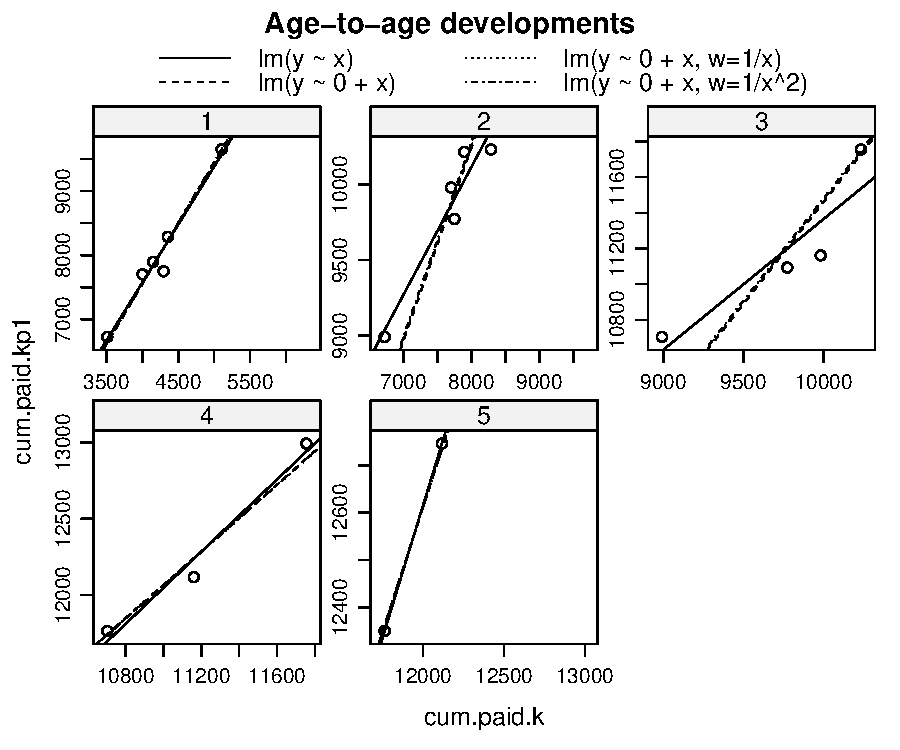
\includegraphics{Log-incremental-linerregressionplot}
\caption{Plot of the cumulative development positions from one development year to the next for each development year, including regression lines of different linear models.}\label{fig:linearregression}
\end{center}
\end{figure}

% \begin{exercise}
% Review the model output
% \end{exercise}


\subsection{Reserving based on log-incremental payments}

%{\bf Warning: from now on, develpement years start at 0}

We noted in the previous section that the claims appear to follow a
log-normal distribution. \cite{Zehnwirth1994} was not the first to consider 
modelling the log of the incremental claims payments, but his papers and software 
ICRFS\footnote{Interactive Claims Reserving and Forecasting System} 
have popularised this  approach. Here we present the key concepts 
of what \cite{Zehnwirth1994} calls the probabilistic trend family (PTF). 

% However, we shall follow the paper of 
% \cite{Christofides1997} more closely, which is part of the Reserving Claims 
% Manual of the Institute of Actuaries.

Zehnwirth's model assumes the following structure for the incremental 
claims $X_{i,j}$
\begin{align} 
\ln(X_{i,j}) & = Y_{i,j} = \alpha_i + \sum_{k=1}^j\gamma_k + 
\sum_{t=1}^{i+j}\iota_t + \varepsilon_{i,j},\label{Zehnwirth} 
\end{align}
The errors are assumed to be normal with $\varepsilon_{i,j} \sim 
\mathcal{N}(0, \sigma^2)$. 
The parameters $\alpha_i, \gamma_j, \iota_t$ model trends in 
three time directions, namely origin year, development year and 
calendar (or payment) year respectively, see Figure~\ref{fig:triangleStructure}. 
%Suppose claims payments would decrease by 50\% every development year,
% \begin{figure}[thb]
% \begin{center}
% \includegraphics{figures/triangle.png}
% \end{center}
% \end{figure}

\begin{figure}[thb]
\begin{center}
\setkeys{Gin}{width=0.3\textwidth}
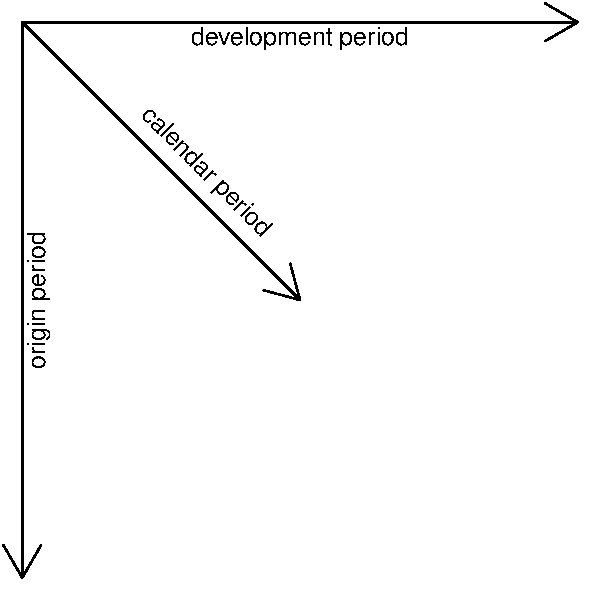
\includegraphics{Log-incremental-trianglestructure}
\caption{Structure of a typical claims triangle and the three time directions: 
origin, development and calendar periods.}
\label{fig:triangleStructure}
\end{center}
\end{figure}

\cite{Christofides1997} examines a very similar model, but uses the following 
notation
\begin{align} 
\ln(X_{i,j}) & = Y_{i,j} = a_i + d_j + \varepsilon_{i,j},
\label{Christofides}
\end{align}
with $a$, $d$ representing the parameters in origin and development period 
direction (a parameter $p_{i+j-1}$ for the payment year direction 
could be added). Although models \ref{Zehnwirth} and \ref{Christofides} 
are essentially the same, the design matrices differ and 
therefore the coefficients and their interpretation.


Note that the above model is not a GLM, e.g. 
$\log(y+\varepsilon)=X\beta$. Instead it models
$\log(y)=X\beta+\varepsilon$; 
although both models assume $\varepsilon \sim \mathcal{N}(0,\sigma^2)$.
Hence, we will use least square regression to fit the coefficients
via \texttt{lm} again.


Before we apply the log-linear model to the data, and we will follow 
\cite{Christofides1997}, we shall plot it again on a log scale.
\begin{Schunk}
\begin{Sinput}
R> Claims <- within(Claims, {
       log.inc <- log(inc.paid.k)
       cal <- as.numeric(levels(originf))[originf] + dev - 1
   })
\end{Sinput}
\end{Schunk}
The interaction plot, Figure~\ref{fig:adjusteddata}, suggests a linear 
relationship  after the second development year on a log-scale. The 
lines of the different origin years are fairly closely group, but the 
last two years, labelled 6 and 7, do stand out. 
We shall test if this is significant.
\begin{figure}[thb]
\begin{center}
\setkeys{Gin}{width=0.75\textwidth}
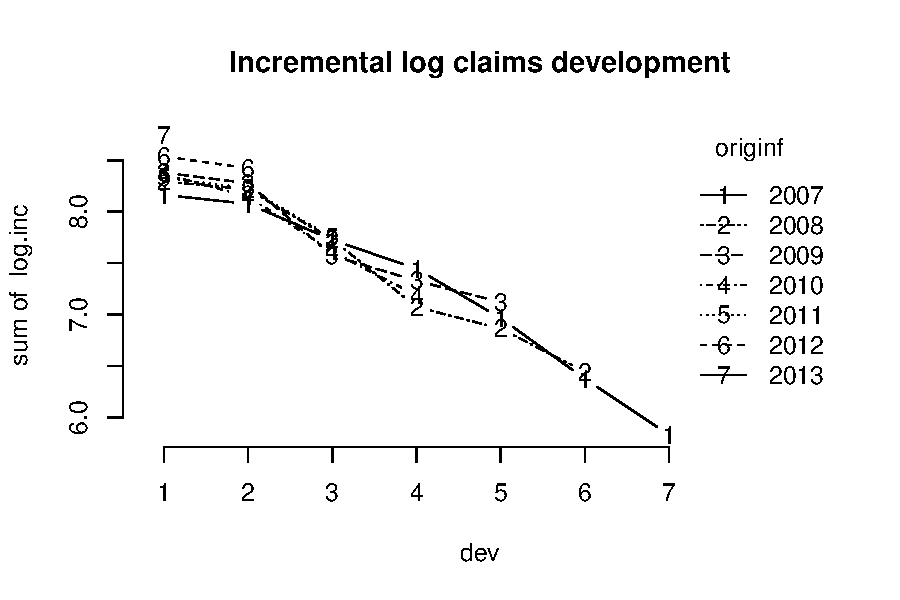
\includegraphics{Log-incremental-019}
\caption{The interaction plot shows the developments of the origin years on a 
log scale. From the second development year the decay appears to be linear.
}\label{fig:adjusteddata}
\end{center}
\end{figure}
We start with a model using all levels of the origin factor 
and two dummy parameters for the development year, with $d_1=d1$ and
$d_j = (j - 1) \cdot d27$ for $j>1$.  
Hence, we add two dummy variables to 
our data.
\begin{Schunk}
\begin{Sinput}
R> Claims <- within(Claims, { 
     d1 <- ifelse(dev < 2, 1, 0)
     d27 <- ifelse(dev < 2, 0, dev - 1)
   })        
\end{Sinput}
\end{Schunk}
The dummy variable $d1$ is $1$ for the first development period and $0$ 
otherwise, while $d27$ is $0$ for the first development period and counts 
up from $1$ then onwards. Hence, we will estimate one parameter for the first 
payment and a constant trend (decay) for the following periods.
% o2012 <- ifelse(origin == 2012, 1, 0)
% o2013 <- ifelse(origin == 2013, 1, 0)
\begin{Schunk}
\begin{Sinput}
R> summary(fit1 <- lm(log.inc ~  originf + d1 + d27, data=Claims))
\end{Sinput}
\begin{Soutput}
Call:
lm(formula = log.inc ~ originf + d1 + d27, data = Claims)

Residuals:
    Min      1Q  Median      3Q     Max 
-0.2214 -0.0397  0.0112  0.0329  0.1962 

Coefficients:
             Estimate Std. Error t value Pr(>|t|)    
(Intercept)  8.572835   0.075690  113.26  < 2e-16 ***
originf2008  0.000956   0.063935    0.01  0.98822    
originf2009  0.092037   0.068675    1.34  0.19600    
originf2010 -0.018715   0.075261   -0.25  0.80629    
originf2011  0.063828   0.084302    0.76  0.45825    
originf2012  0.272668   0.098245    2.78  0.01205 *  
originf2013  0.468983   0.131593    3.56  0.00207 ** 
d1          -0.296215   0.069903   -4.24  0.00045 ***
d27         -0.434960   0.018488  -23.53  1.6e-15 ***
---
Signif. codes:  0 ‘***’ 0.001 ‘**’ 0.01 ‘*’ 0.05 ‘.’ 0.1 ‘ ’ 1

Residual standard error: 0.114 on 19 degrees of freedom
Multiple R-squared:  0.983,	Adjusted R-squared:  0.976 
F-statistic:  139 on 8 and 19 DF,  p-value: 3.29e-15
\end{Soutput}
\end{Schunk}
The model output confirms what we had noticed from the interaction
plot already, apart from the origin years 2012 and 2013 there is no 
significant difference between the years; the p-values are all greater than 5\% and
the coefficients are less than twice their standard errors. 
Therefore we reduce the model and replace the origin variable with two dummy 
columns for those years.
% ff=Claims$origin
% levels(ff)=c(rep('base',5), '2012', 2013)
% summary(Fit2 <- lm(log.inc ~ ff + d1 + d27, data=Claims))
\begin{Schunk}
\begin{Sinput}
R> Claims <- within(Claims, { 
     a6 <- ifelse(originf == 2012, 1, 0)
     a7 <- ifelse(originf == 2013, 1, 0)
   })
R> summary(fit2 <- lm(log.inc ~  a6 + a7 + d1 + d27, data=Claims))
\end{Sinput}
\begin{Soutput}
Call:
lm(formula = log.inc ~ a6 + a7 + d1 + d27, data = Claims)

Residuals:
     Min       1Q   Median       3Q      Max 
-0.21567 -0.04910  0.00654  0.05137  0.27199 

Coefficients:
            Estimate Std. Error t value Pr(>|t|)    
(Intercept)   8.6079     0.0515  167.14  < 2e-16 ***
a6            0.2435     0.0852    2.86  0.00887 ** 
a7            0.4411     0.1217    3.62  0.00142 ** 
d1           -0.3035     0.0678   -4.48  0.00017 ***
d27          -0.4397     0.0167  -26.39  < 2e-16 ***
---
Signif. codes:  0 ‘***’ 0.001 ‘**’ 0.01 ‘*’ 0.05 ‘.’ 0.1 ‘ ’ 1

Residual standard error: 0.112 on 23 degrees of freedom
Multiple R-squared:  0.98,	Adjusted R-squared:  0.977 
F-statistic:  288 on 4 and 23 DF,  p-value: <2e-16
\end{Soutput}
\end{Schunk}
% summary(fit2 <- update(fit1, ~ . + a6 + a7 - origin, data=Claims))
The reduction in parameters from 9 to 5 seems sensible, all coefficient 
are significant and the model error reduced from 
0.114 to 0.112 as 
well.  Further we can read off the coefficient for $d27$ that claims 
payments are predicted to reduce by 44\% each year after year one.
Next, we plot the model:
\begin{Schunk}
\begin{Sinput}
R> op <- par(mfrow=c(2,2), oma = c(0, 0, 3, 0))
R> plot(fit2)
R> par(op)
\end{Sinput}
\end{Schunk}
Reviewing the residual plots in Figure~\ref{fig:fit2plot2} highlights 
again the latest payment for the 2009 origin year (the 18th row of the 
Claims data) as a potential outlier.

The error distribution  appears to follow a normal distribution, top right 
qq-plot in Figure~\ref{fig:fit2plot2}, confirmed by the Shapiro-Wilk normality test. 
\begin{Schunk}
\begin{Sinput}
R> shapiro.test(fit2$residuals)
\end{Sinput}
\begin{Soutput}
	Shapiro-Wilk normality test

data:  fit2$residuals
W = 0.97, p-value = 0.5
\end{Soutput}
\end{Schunk}

\begin{figure}[thb]
\begin{center}
\setkeys{Gin}{width=0.75\textwidth}
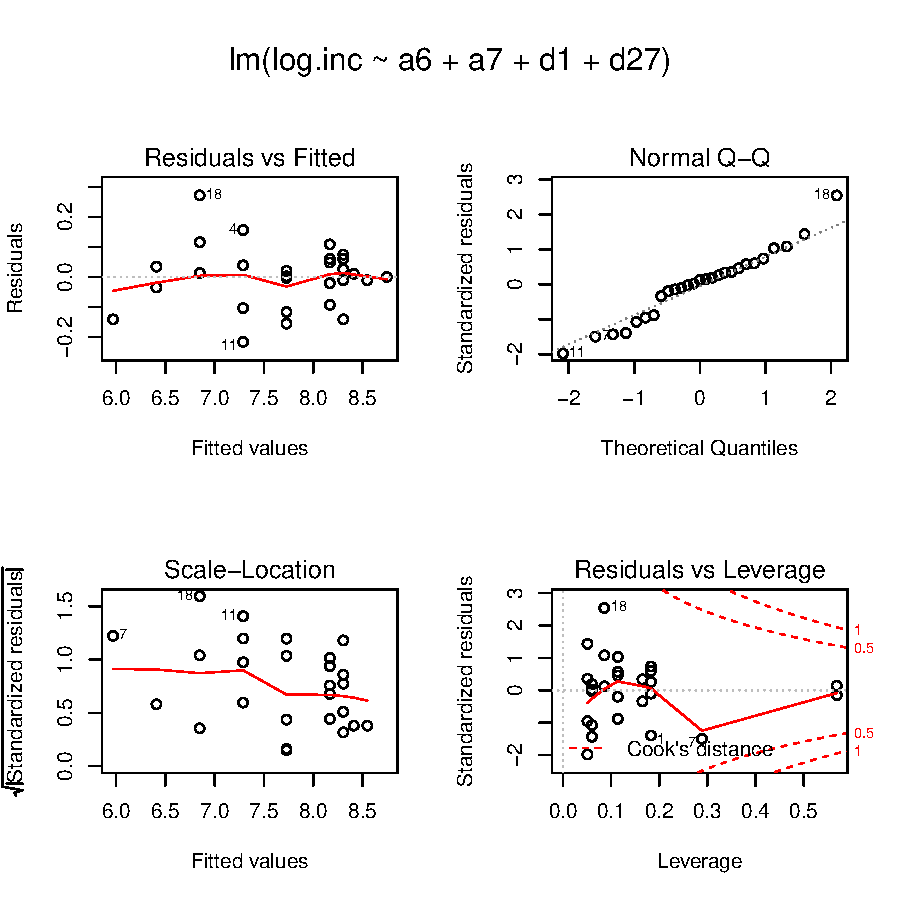
\includegraphics{Log-incremental-025}
\caption{Residual plots of the log-incremental model \texttt{fit2}.
The last payment of 2009 (row 18) is highlighted again as a potential outlier, 
so are rows 11, 7 and 4.}\label{fig:fit2plot2}
\end{center}
\end{figure}
% We can test as well if the resdiuals are distributed normally.
% <<>>=
% shapiro.test(fit2$residuals)
% @
% The Shapiro-Wilk test doesn't reject the null hypothesis that the 
% residuals are normally distributed. 
To investigate the residuals further we shall plot them against the 
fitted values and the three trend directions. 
The following function will create those four plots for our 
model.
\begin{Schunk}
\begin{Sinput}
R> resPlot <- function(model, data){
     xvals <- list(
       fitted = model[['fitted.values']],
       origin = as.numeric(levels(data$originf))[data$originf],
       cal=data$cal, dev=data$dev
     )
     op <- par(mfrow=c(2,2), oma = c(0, 0, 3, 0))
     for(i in 1:4){
     plot.default(rstandard(model) ~ xvals[[i]] ,
                  main=paste("Residuals vs", names(xvals)[i] ),
                  xlab=names(xvals)[i], ylab="Standardized residuals")
     panel.smooth(y=rstandard(model), x=xvals[[i]])
     abline(h=0, lty=2)
     }
     mtext(as.character(model$call)[2], outer = TRUE, cex = 1.2)
     par(op)
   }
\end{Sinput}
\end{Schunk}
\begin{Schunk}
\begin{Sinput}
R> resPlot(fit2, Claims)
\end{Sinput}
\end{Schunk}
\begin{figure}[thb]
\begin{center}
\setkeys{Gin}{width=0.75\textwidth}
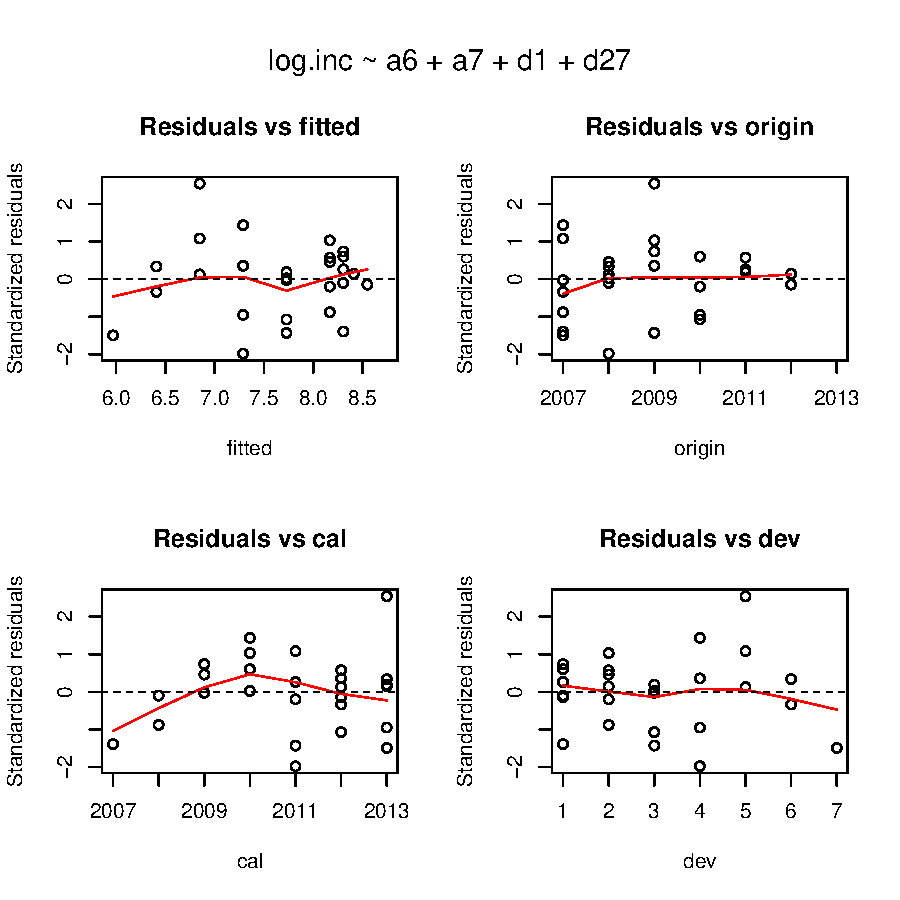
\includegraphics{Log-incremental-028}
\caption{Residual plots of the log-incremental model \texttt{fit2} against 
fitted values and the three trend directions.}\label{fig:fit2plot}
\end{center}
\end{figure}
Again, the residual plots all look fairly well behaved, 
however, we notice from the bottom left plot in Figure~\ref{fig:fit2plot} 
that claims for the payment years 2007, 2008 are slightly over-fitted and 
2009, 2010 are under-fitted. Hence, we introduce an additional parameter 
for that period and update our model.
\begin{Schunk}
\begin{Sinput}
R> Claims <- within(Claims, { 
     p34 <- ifelse(cal < 2011 & cal > 2008, cal-2008, 0)
   })
R> summary(fit3 <- update(fit2, ~  . + p34, data=Claims))
\end{Sinput}
\begin{Soutput}
Call:
lm(formula = log.inc ~ a6 + a7 + d1 + d27 + p34, data = Claims)

Residuals:
    Min      1Q  Median      3Q     Max 
-0.1941 -0.0595  0.0164  0.0511  0.2840 

Coefficients:
            Estimate Std. Error t value Pr(>|t|)    
(Intercept)   8.5576     0.0540  158.51  < 2e-16 ***
a6            0.2822     0.0819    3.45  0.00230 ** 
a7            0.4777     0.1152    4.15  0.00042 ***
d1           -0.2897     0.0638   -4.54  0.00016 ***
d27          -0.4301     0.0163  -26.45  < 2e-16 ***
p34           0.0603     0.0292    2.07  0.05074 .  
---
Signif. codes:  0 ‘***’ 0.001 ‘**’ 0.01 ‘*’ 0.05 ‘.’ 0.1 ‘ ’ 1

Residual standard error: 0.105 on 22 degrees of freedom
Multiple R-squared:  0.984,	Adjusted R-squared:  0.98 
F-statistic:  264 on 5 and 22 DF,  p-value: <2e-16
\end{Soutput}
\end{Schunk}
\begin{Schunk}
\begin{Sinput}
R> resPlot(fit3, Claims)
\end{Sinput}
\end{Schunk}
The residual plot against calendar years, Figure~\ref{fig:fit3plot}, has 
improved and the parameter $p34$ could be regarded significant.
The coefficient $p34$ describes a 6\% increase of claims payments in those two 
years. An investigation should clarify if this effect is the result of a 
temporary increase in claims  inflation, a change in the claims settling 
process, other causes or just random noise.
Observe that the new model has a slightly lower residual standard error of 
0.105 compared to 0.112. 
\begin{figure}[thb]
\begin{center}
\setkeys{Gin}{width=0.75\textwidth}
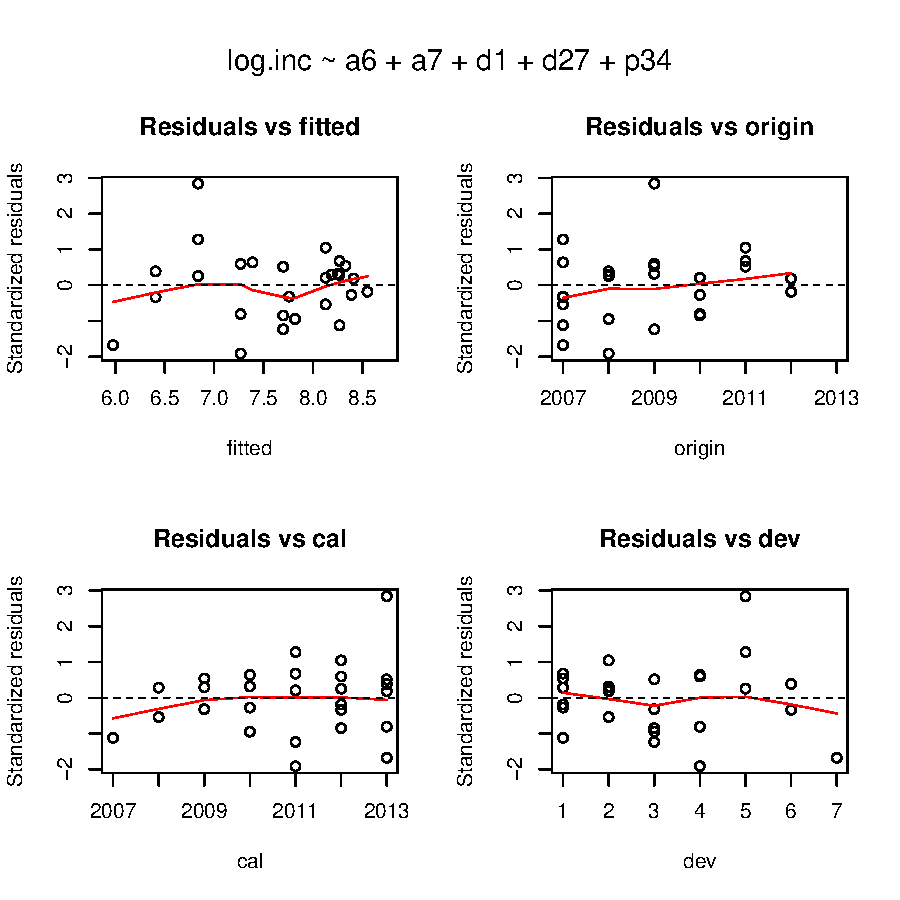
\includegraphics{Log-incremental-031}
\caption{Residual plot of the log-incremental model \texttt{fit3}.}\label{fig:fit3plot}
\end{center}
\end{figure}
% Test the model by taking the latest calendar year data out
% <<>>=
% Fit3_2012 <- update(Fit3, data=subset(Claims, cal <= 2012))
% testCoef <- cbind(summary(Fit3)$coefficients[,1:2], 
%                   summary(Fit3_2012)$coefficients[,1:2])
% colnames(testCoef)[c(1,3)] <- paste("Up to", 2012:2013)
% testCoef
% @

Within the linear regression framework we can forecast the claims
payments and estimated the standard errors. We follow the paper by 
\cite{Christofides1997} again. Recall that for a log-normal distribution the mean
is $E(X) = \exp(\mu + 1/2 \sigma^2)$ and the variance is
$Var(X) = \exp(2\mu + \sigma^2)(\exp(\sigma^2) - 1)$,
where $\mu$ and $\sigma$ are the mean and standard deviation of the logarithm.
\begin{Schunk}
\begin{Sinput}
R> log.incr.predict <- function(model, newdata){
     Pred <- predict(model, newdata=newdata, se.fit=TRUE)  
     Y <- Pred$fit
     VarY <- Pred$se.fit^2 + Pred$residual.scale^2 
     P <- exp(Y + VarY/2)
     VarP <-  P^2*(exp(VarY)-1)
     seP <- sqrt(VarP)
     model.formula <- as.formula(paste("~", formula(model)[3]))
     mframe <- model.frame(model.formula, data=newdata)
     X <- model.matrix(model.formula, data=newdata)
     varcovar <- X %*% vcov(model) %*% t(X)
     CoVar <-  sweep(sweep((exp(varcovar)-1), 1, P, "*"), 2, P, "*")
     CoVar[col(CoVar)==row(CoVar)] <- 0 
     Total.SE <- sqrt(sum(CoVar) + sum(VarP))
     Total.Reserve <- sum(P)
     Incr=data.frame(newdata, Y, VarY, P, seP, CV=seP/P)
     out <- list(Forecast=Incr,              
                 Totals=data.frame(Total.Reserve, 
                                   Total.SE=Total.SE, 
                                   CV=Total.SE/Total.Reserve))
     return(out)
   }
\end{Sinput}
\end{Schunk}
% Z <- t(P) %*% (exp(varcovar)) %*% P
% Total.SE <- sqrt(Z + sum(VarP))
With the above function it is straightforward to carry out the
prediction for future claims payment and standard errors. 
As a bonus we can estimate payments beyond the available data.

To forecast the future claims we prepare a data frame with the 
predictors for those years, here with 6 years beyond age 7. 
\begin{Schunk}
\begin{Sinput}
R> tail.years <-6
R> fdat <- data.frame(
     origin=rep(2007:2013, n+tail.years),
     dev=rep(1:(n+tail.years), each=n)
     )
R> fdat <- within(fdat, {
     cal <- origin + dev - 1
     a7 <- ifelse(origin == 2013, 1, 0)
     a6 <- ifelse(origin == 2012, 1, 0)
     originf <- factor(origin)
     p34 <- ifelse(cal < 2011 & cal > 2008, cal-2008, 0)
     d1 <- ifelse(dev < 2, 1, 0)
     d27 <- ifelse(dev < 2, 0, dev - 1)
   })  
\end{Sinput}
\end{Schunk}
So, here are the results for the two models:
\begin{Schunk}
\begin{Sinput}
R> reserve2 <- log.incr.predict(fit2, subset(fdat, cal>2013))
R> reserve2$Totals 
\end{Sinput}
\begin{Soutput}
  Total.Reserve Total.SE      CV
1         33847     2545 0.07519
\end{Soutput}
\begin{Sinput}
R> reserve3 <- log.incr.predict(fit3, subset(fdat, cal>2013))
R> reserve3$Totals
\end{Sinput}
\begin{Soutput}
  Total.Reserve Total.SE      CV
1         34251     2424 0.07078
\end{Soutput}
\end{Schunk}
The two models produce very similar results and it shouldn't be much
of a surprise as they are quite similar indeed. The third model has 
proportionally a slightly smaller standard error and may hence 
be the preferred choice.  

The future payments can be displayed with the \texttt{xtabs} function:
\begin{Schunk}
\begin{Sinput}
R> round(xtabs(P ~ origin + dev, reserve3$Forecast))
\end{Sinput}
\begin{Soutput}
      dev
origin    2    3    4    5    6    7    8    9   10   11   12   13
  2007    0    0    0    0    0    0  259  168  110   71   47   30
  2008    0    0    0    0    0  397  259  168  110   71   47   30
  2009    0    0    0    0  610  397  259  168  110   71   47   30
  2010    0    0    0  937  610  397  259  168  110   71   47   30
  2011    0    0 1441  937  610  397  259  168  110   71   47   30
  2012    0 2946 1916 1247  812  529  344  224  146   95   62   40
  2013 5529 3595 2338 1521  990  645  420  273  178  116   76   49
\end{Soutput}
\end{Schunk}
The model structure is clearly visible in the above future claims triangle; as 
the origin years 2007 to 2011 share the same parameter, the predicted future 
payments for those years have the same identical mean expectations.

For comparison here is the output of the Mack chain-ladder model, assuming a
tail factor of 1.05 and standard error of 0.02: 
\begin{Schunk}
\begin{Sinput}
R> round(summary(MackChainLadder(cum.triangle, est.sigma="Mack",
                        tail=1.05, tail.se=0.02))$Totals,2)
\end{Sinput}
\begin{Soutput}
              Totals
Latest:     75672.00
Dev:            0.69
Ultimate:  109544.16
IBNR:       33872.16
Mack S.E.:   2563.40
CV(IBNR):       0.08
\end{Soutput}
\end{Schunk}
The chain ladder method provides similar forecast to the
log-incremental regression model, but at the price of many more
parameters and hence potential instability. 

A model with few parameters is potentially more robust and can be analysed by
back testing the model with fewer data points.

The log-incremental regression model provides an intuitive 
and elegant stochastic claims reserving model and can help to investigate 
trends in the calendar/payment year direction, such as claims inflation, which is
challenging to define and measure, \cite{GesmannRayeesClapham2013}. 
%Those trend changes can highlight movements in claims inflation, 
%or indeed changes in the claims settling process. 
%Neither of those factors should be ignored. 
Additionally the tail extrapolation is part of the model design and not a 
artificial add on. 

See \cite{Christofides1997} and \cite{Zehnwirth1994} for a more detailed 
discussion of the log-incremental model.

\bibliographystyle{plain}
\bibliography{Chapter_15}

\end{document}
